\section{Durchführung und Aufbau}
\label{sec:Durchführung}

\subsection{Messung der Hall-Spannung}
Für die Messung der Hallspannung in Abhängigkeit des Querstroms $I_\text{q}$ wird der Aufbau aus Abbildung \eqref{fig:Hall-Aufbau} verwendet.

\begin{figure}[H]
  \centering
  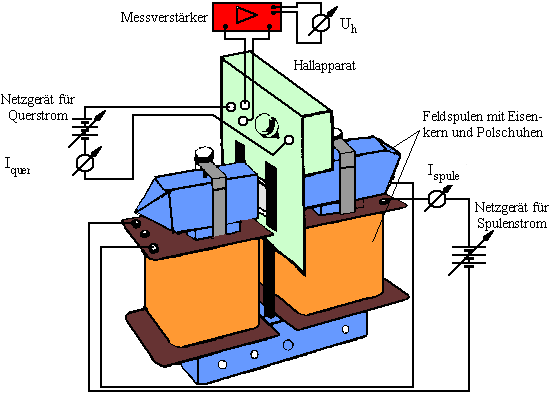
\includegraphics[height=7cm]{picture/Hall-Aufbau.PNG}
  \caption{Versuchsaufbau zur Messung der Hall-Spannung. \cite{Leifi}}
  \label{fig:Hall-Aufbau}
\end{figure}
